% Created by tikzDevice version 0.12.6 on 2026-08-03 04:42:11
% !TEX encoding = UTF-8 Unicode
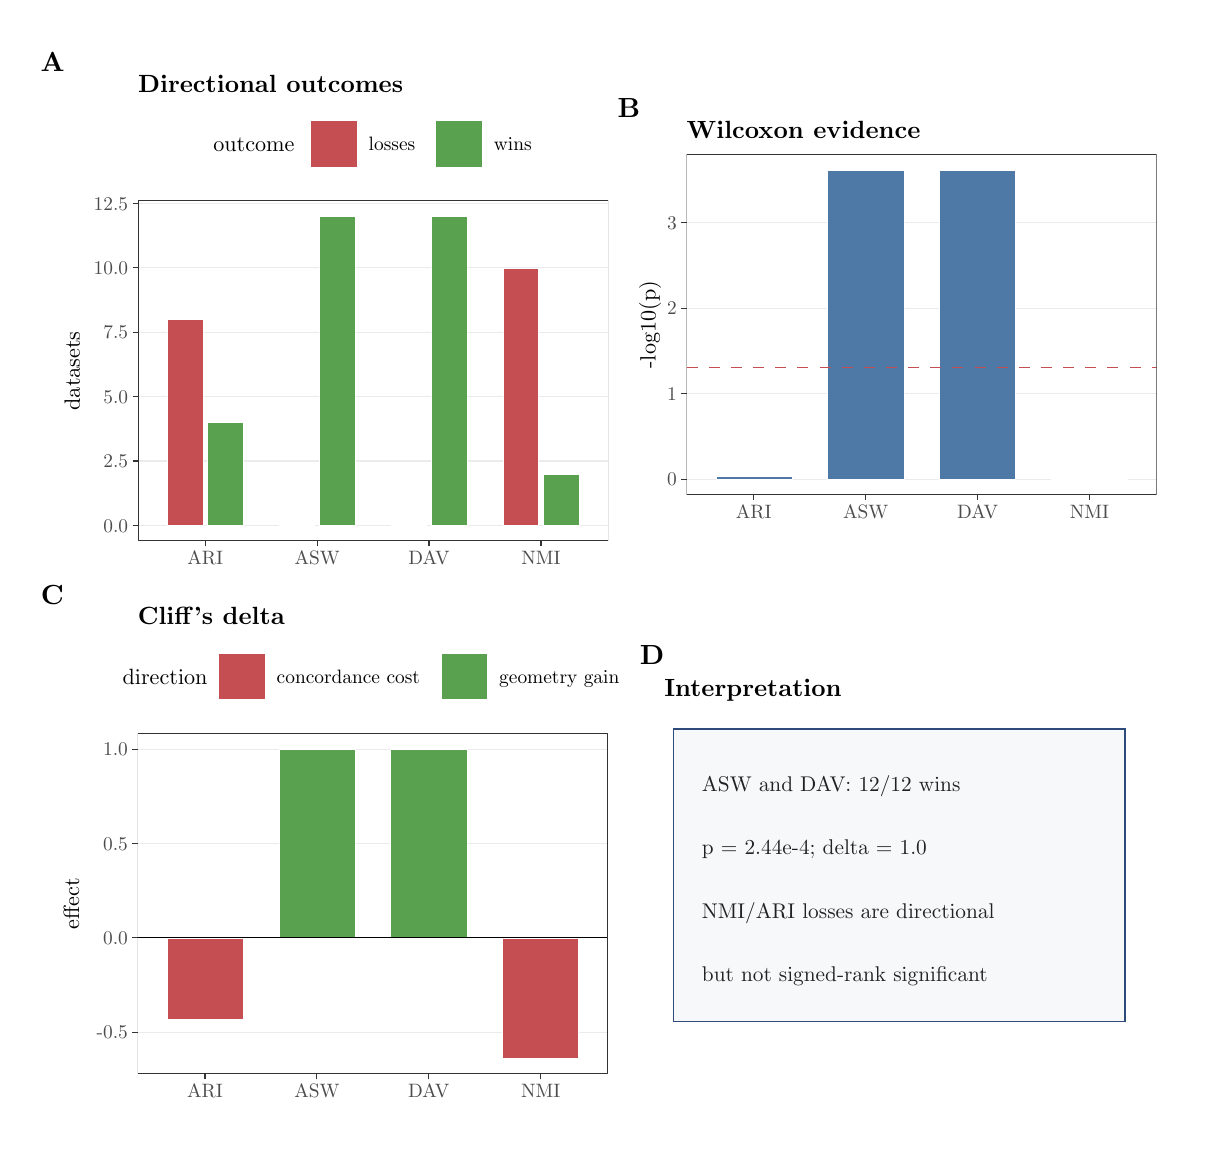
\begin{tikzpicture}[x=1pt,y=1pt]
\definecolor{fillColor}{RGB}{255,255,255}
\path[use as bounding box,fill=fillColor,fill opacity=0.00] (0,0) rectangle (417.77,396.13);
\begin{scope}
\path[clip] (  0.00,  0.00) rectangle (417.77,396.13);
\definecolor{drawColor}{RGB}{255,255,255}
\definecolor{fillColor}{RGB}{255,255,255}

\path[draw=drawColor,line width= 0.6pt,line join=round,line cap=round,fill=fillColor] (  0.00,  0.00) rectangle (417.77,396.13);
\end{scope}
\begin{scope}
\path[clip] (  5.50,198.06) rectangle (208.88,390.63);
\definecolor{drawColor}{RGB}{255,255,255}
\definecolor{fillColor}{RGB}{255,255,255}

\path[draw=drawColor,line width= 0.6pt,line join=round,line cap=round,fill=fillColor] (  5.50,198.06) rectangle (208.88,390.63);
\end{scope}
\begin{scope}
\path[clip] (208.88,198.06) rectangle (412.27,390.63);
\definecolor{drawColor}{RGB}{255,255,255}
\definecolor{fillColor}{RGB}{255,255,255}

\path[draw=drawColor,line width= 0.6pt,line join=round,line cap=round,fill=fillColor] (208.88,198.06) rectangle (412.27,390.63);
\end{scope}
\begin{scope}
\path[clip] (  2.65,198.50) rectangle (211.73,390.20);
\definecolor{drawColor}{RGB}{255,255,255}
\definecolor{fillColor}{RGB}{255,255,255}

\path[draw=drawColor,line width= 0.4pt,line join=round,line cap=round,fill=fillColor] (  2.65,198.50) rectangle (211.73,390.20);
\end{scope}
\begin{scope}
\path[clip] ( 39.90,210.69) rectangle (209.73,333.55);
\definecolor{fillColor}{RGB}{255,255,255}

\path[fill=fillColor] ( 39.90,210.69) rectangle (209.73,333.55);
\definecolor{drawColor}{gray}{0.92}

\path[draw=drawColor,line width= 0.4pt,line join=round] ( 39.90,216.27) --
	(209.73,216.27);

\path[draw=drawColor,line width= 0.4pt,line join=round] ( 39.90,239.54) --
	(209.73,239.54);

\path[draw=drawColor,line width= 0.4pt,line join=round] ( 39.90,262.81) --
	(209.73,262.81);

\path[draw=drawColor,line width= 0.4pt,line join=round] ( 39.90,286.08) --
	(209.73,286.08);

\path[draw=drawColor,line width= 0.4pt,line join=round] ( 39.90,309.35) --
	(209.73,309.35);

\path[draw=drawColor,line width= 0.4pt,line join=round] ( 39.90,332.62) --
	(209.73,332.62);
\definecolor{drawColor}{RGB}{255,255,255}
\definecolor{fillColor}{RGB}{89,161,79}

\path[draw=drawColor,line width= 0.2pt,fill=fillColor] (186.28,216.27) rectangle (199.22,234.89);

\path[draw=drawColor,line width= 0.2pt,fill=fillColor] ( 64.97,216.27) rectangle ( 77.91,253.50);

\path[draw=drawColor,line width= 0.2pt,fill=fillColor] (105.40,216.27) rectangle (118.34,327.96);

\path[draw=drawColor,line width= 0.2pt,fill=fillColor] (145.84,216.27) rectangle (158.78,327.96);
\definecolor{fillColor}{RGB}{196,78,82}

\path[draw=drawColor,line width= 0.2pt,fill=fillColor] (171.72,216.27) rectangle (184.66,309.35);

\path[draw=drawColor,line width= 0.2pt,fill=fillColor] ( 50.41,216.27) rectangle ( 63.35,290.73);

\path[draw=drawColor,line width= 0.2pt,fill=fillColor] ( 90.85,216.27) rectangle (103.79,216.27);

\path[draw=drawColor,line width= 0.2pt,fill=fillColor] (131.28,216.27) rectangle (144.22,216.27);
\definecolor{drawColor}{gray}{0.20}

\path[draw=drawColor,line width= 0.4pt,line join=round,line cap=round] ( 39.90,210.69) rectangle (209.73,333.55);
\end{scope}
\begin{scope}
\path[clip] (  0.00,  0.00) rectangle (417.77,396.13);
\definecolor{drawColor}{gray}{0.30}

\node[text=drawColor,anchor=base east,inner sep=0pt, outer sep=0pt, scale=  0.70] at ( 36.30,213.86) {0.0};

\node[text=drawColor,anchor=base east,inner sep=0pt, outer sep=0pt, scale=  0.70] at ( 36.30,237.13) {2.5};

\node[text=drawColor,anchor=base east,inner sep=0pt, outer sep=0pt, scale=  0.70] at ( 36.30,260.40) {5.0};

\node[text=drawColor,anchor=base east,inner sep=0pt, outer sep=0pt, scale=  0.70] at ( 36.30,283.67) {7.5};

\node[text=drawColor,anchor=base east,inner sep=0pt, outer sep=0pt, scale=  0.70] at ( 36.30,306.94) {10.0};

\node[text=drawColor,anchor=base east,inner sep=0pt, outer sep=0pt, scale=  0.70] at ( 36.30,330.20) {12.5};
\end{scope}
\begin{scope}
\path[clip] (  0.00,  0.00) rectangle (417.77,396.13);
\definecolor{drawColor}{gray}{0.20}

\path[draw=drawColor,line width= 0.4pt,line join=round] ( 37.90,216.27) --
	( 39.90,216.27);

\path[draw=drawColor,line width= 0.4pt,line join=round] ( 37.90,239.54) --
	( 39.90,239.54);

\path[draw=drawColor,line width= 0.4pt,line join=round] ( 37.90,262.81) --
	( 39.90,262.81);

\path[draw=drawColor,line width= 0.4pt,line join=round] ( 37.90,286.08) --
	( 39.90,286.08);

\path[draw=drawColor,line width= 0.4pt,line join=round] ( 37.90,309.35) --
	( 39.90,309.35);

\path[draw=drawColor,line width= 0.4pt,line join=round] ( 37.90,332.62) --
	( 39.90,332.62);
\end{scope}
\begin{scope}
\path[clip] (  0.00,  0.00) rectangle (417.77,396.13);
\definecolor{drawColor}{gray}{0.20}

\path[draw=drawColor,line width= 0.4pt,line join=round] ( 64.16,208.69) --
	( 64.16,210.69);

\path[draw=drawColor,line width= 0.4pt,line join=round] (104.59,208.69) --
	(104.59,210.69);

\path[draw=drawColor,line width= 0.4pt,line join=round] (145.03,208.69) --
	(145.03,210.69);

\path[draw=drawColor,line width= 0.4pt,line join=round] (185.47,208.69) --
	(185.47,210.69);
\end{scope}
\begin{scope}
\path[clip] (  0.00,  0.00) rectangle (417.77,396.13);
\definecolor{drawColor}{gray}{0.30}

\node[text=drawColor,anchor=base,inner sep=0pt, outer sep=0pt, scale=  0.70] at ( 64.16,202.27) {ARI};

\node[text=drawColor,anchor=base,inner sep=0pt, outer sep=0pt, scale=  0.70] at (104.59,202.27) {ASW};

\node[text=drawColor,anchor=base,inner sep=0pt, outer sep=0pt, scale=  0.70] at (145.03,202.27) {DAV};

\node[text=drawColor,anchor=base,inner sep=0pt, outer sep=0pt, scale=  0.70] at (185.47,202.27) {NMI};
\end{scope}
\begin{scope}
\path[clip] (  0.00,  0.00) rectangle (417.77,396.13);
\definecolor{drawColor}{RGB}{0,0,0}

\node[text=drawColor,rotate= 90.00,anchor=base,inner sep=0pt, outer sep=0pt, scale=  0.80] at ( 18.86,272.12) {datasets};
\end{scope}
\begin{scope}
\path[clip] (  0.00,  0.00) rectangle (417.77,396.13);
\definecolor{fillColor}{RGB}{255,255,255}

\path[fill=fillColor] ( 63.09,341.55) rectangle (186.54,366.89);
\end{scope}
\begin{scope}
\path[clip] (  0.00,  0.00) rectangle (417.77,396.13);
\definecolor{drawColor}{RGB}{0,0,0}

\node[text=drawColor,anchor=base west,inner sep=0pt, outer sep=0pt, scale=  0.80] at ( 67.09,351.46) {outcome};
\end{scope}
\begin{scope}
\path[clip] (  0.00,  0.00) rectangle (417.77,396.13);
\definecolor{fillColor}{RGB}{255,255,255}

\path[fill=fillColor] (101.88,345.55) rectangle (119.23,362.89);
\definecolor{drawColor}{RGB}{255,255,255}
\definecolor{fillColor}{RGB}{196,78,82}

\path[draw=drawColor,line width= 0.2pt,fill=fillColor] (102.17,345.83) rectangle (118.94,362.61);
\end{scope}
\begin{scope}
\path[clip] (  0.00,  0.00) rectangle (417.77,396.13);
\definecolor{fillColor}{RGB}{255,255,255}

\path[fill=fillColor] (147.14,345.55) rectangle (164.48,362.89);
\definecolor{drawColor}{RGB}{255,255,255}
\definecolor{fillColor}{RGB}{89,161,79}

\path[draw=drawColor,line width= 0.2pt,fill=fillColor] (147.42,345.83) rectangle (164.20,362.61);
\end{scope}
\begin{scope}
\path[clip] (  0.00,  0.00) rectangle (417.77,396.13);
\definecolor{drawColor}{RGB}{0,0,0}

\node[text=drawColor,anchor=base west,inner sep=0pt, outer sep=0pt, scale=  0.70] at (123.23,351.81) {losses};
\end{scope}
\begin{scope}
\path[clip] (  0.00,  0.00) rectangle (417.77,396.13);
\definecolor{drawColor}{RGB}{0,0,0}

\node[text=drawColor,anchor=base west,inner sep=0pt, outer sep=0pt, scale=  0.70] at (168.48,351.81) {wins};
\end{scope}
\begin{scope}
\path[clip] (  0.00,  0.00) rectangle (417.77,396.13);
\definecolor{drawColor}{RGB}{0,0,0}

\node[text=drawColor,anchor=base west,inner sep=0pt, outer sep=0pt, scale=  0.90] at ( 39.90,372.88) {\bfseries Directional outcomes};
\end{scope}
\begin{scope}
\path[clip] (  0.00,  0.00) rectangle (417.77,396.13);
\definecolor{drawColor}{RGB}{0,0,0}

\node[text=drawColor,anchor=base,inner sep=0pt, outer sep=0pt, scale=  1.00] at (  9.00,380.19) {\bfseries A};
\end{scope}
\begin{scope}
\path[clip] (211.18,215.17) rectangle (409.97,373.53);
\definecolor{drawColor}{RGB}{255,255,255}
\definecolor{fillColor}{RGB}{255,255,255}

\path[draw=drawColor,line width= 0.4pt,line join=round,line cap=round,fill=fillColor] (211.18,215.17) rectangle (409.97,373.53);
\end{scope}
\begin{scope}
\path[clip] (238.14,227.36) rectangle (407.97,350.22);
\definecolor{fillColor}{RGB}{255,255,255}

\path[fill=fillColor] (238.14,227.36) rectangle (407.97,350.22);
\definecolor{drawColor}{gray}{0.92}

\path[draw=drawColor,line width= 0.4pt,line join=round] (238.14,232.94) --
	(407.97,232.94);

\path[draw=drawColor,line width= 0.4pt,line join=round] (238.14,263.86) --
	(407.97,263.86);

\path[draw=drawColor,line width= 0.4pt,line join=round] (238.14,294.78) --
	(407.97,294.78);

\path[draw=drawColor,line width= 0.4pt,line join=round] (238.14,325.69) --
	(407.97,325.69);
\definecolor{drawColor}{RGB}{255,255,255}
\definecolor{fillColor}{RGB}{78,121,167}

\path[draw=drawColor,line width= 0.2pt,fill=fillColor] (369.96,232.94) rectangle (397.46,232.96);

\path[draw=drawColor,line width= 0.2pt,fill=fillColor] (248.65,232.94) rectangle (276.15,234.01);

\path[draw=drawColor,line width= 0.2pt,fill=fillColor] (289.09,232.94) rectangle (316.59,344.63);

\path[draw=drawColor,line width= 0.2pt,fill=fillColor] (329.53,232.94) rectangle (357.02,344.63);
\definecolor{drawColor}{RGB}{196,78,82}

\path[draw=drawColor,line width= 0.4pt,dash pattern=on 4pt off 4pt ,line join=round] (238.14,273.17) -- (407.97,273.17);
\definecolor{drawColor}{gray}{0.20}

\path[draw=drawColor,line width= 0.4pt,line join=round,line cap=round] (238.14,227.36) rectangle (407.97,350.22);
\end{scope}
\begin{scope}
\path[clip] (  0.00,  0.00) rectangle (417.77,396.13);
\definecolor{drawColor}{gray}{0.30}

\node[text=drawColor,anchor=base east,inner sep=0pt, outer sep=0pt, scale=  0.70] at (234.54,230.53) {0};

\node[text=drawColor,anchor=base east,inner sep=0pt, outer sep=0pt, scale=  0.70] at (234.54,261.45) {1};

\node[text=drawColor,anchor=base east,inner sep=0pt, outer sep=0pt, scale=  0.70] at (234.54,292.37) {2};

\node[text=drawColor,anchor=base east,inner sep=0pt, outer sep=0pt, scale=  0.70] at (234.54,323.28) {3};
\end{scope}
\begin{scope}
\path[clip] (  0.00,  0.00) rectangle (417.77,396.13);
\definecolor{drawColor}{gray}{0.20}

\path[draw=drawColor,line width= 0.4pt,line join=round] (236.14,232.94) --
	(238.14,232.94);

\path[draw=drawColor,line width= 0.4pt,line join=round] (236.14,263.86) --
	(238.14,263.86);

\path[draw=drawColor,line width= 0.4pt,line join=round] (236.14,294.78) --
	(238.14,294.78);

\path[draw=drawColor,line width= 0.4pt,line join=round] (236.14,325.69) --
	(238.14,325.69);
\end{scope}
\begin{scope}
\path[clip] (  0.00,  0.00) rectangle (417.77,396.13);
\definecolor{drawColor}{gray}{0.20}

\path[draw=drawColor,line width= 0.4pt,line join=round] (262.40,225.36) --
	(262.40,227.36);

\path[draw=drawColor,line width= 0.4pt,line join=round] (302.84,225.36) --
	(302.84,227.36);

\path[draw=drawColor,line width= 0.4pt,line join=round] (343.27,225.36) --
	(343.27,227.36);

\path[draw=drawColor,line width= 0.4pt,line join=round] (383.71,225.36) --
	(383.71,227.36);
\end{scope}
\begin{scope}
\path[clip] (  0.00,  0.00) rectangle (417.77,396.13);
\definecolor{drawColor}{gray}{0.30}

\node[text=drawColor,anchor=base,inner sep=0pt, outer sep=0pt, scale=  0.70] at (262.40,218.94) {ARI};

\node[text=drawColor,anchor=base,inner sep=0pt, outer sep=0pt, scale=  0.70] at (302.84,218.94) {ASW};

\node[text=drawColor,anchor=base,inner sep=0pt, outer sep=0pt, scale=  0.70] at (343.27,218.94) {DAV};

\node[text=drawColor,anchor=base,inner sep=0pt, outer sep=0pt, scale=  0.70] at (383.71,218.94) {NMI};
\end{scope}
\begin{scope}
\path[clip] (  0.00,  0.00) rectangle (417.77,396.13);
\definecolor{drawColor}{RGB}{0,0,0}

\node[text=drawColor,rotate= 90.00,anchor=base,inner sep=0pt, outer sep=0pt, scale=  0.80] at (226.87,288.79) {-log10(p)};
\end{scope}
\begin{scope}
\path[clip] (  0.00,  0.00) rectangle (417.77,396.13);
\definecolor{drawColor}{RGB}{0,0,0}

\node[text=drawColor,anchor=base west,inner sep=0pt, outer sep=0pt, scale=  0.90] at (238.14,356.21) {\bfseries Wilcoxon evidence};
\end{scope}
\begin{scope}
\path[clip] (  0.00,  0.00) rectangle (417.77,396.13);
\definecolor{drawColor}{RGB}{0,0,0}

\node[text=drawColor,anchor=base,inner sep=0pt, outer sep=0pt, scale=  1.00] at (217.27,363.52) {\bfseries B};
\end{scope}
\begin{scope}
\path[clip] (  5.50,  5.50) rectangle (208.88,198.06);
\definecolor{drawColor}{RGB}{255,255,255}
\definecolor{fillColor}{RGB}{255,255,255}

\path[draw=drawColor,line width= 0.6pt,line join=round,line cap=round,fill=fillColor] (  5.50,  5.50) rectangle (208.88,198.06);
\end{scope}
\begin{scope}
\path[clip] (208.88,  5.50) rectangle (412.27,198.06);
\definecolor{drawColor}{RGB}{255,255,255}
\definecolor{fillColor}{RGB}{255,255,255}

\path[draw=drawColor,line width= 0.6pt,line join=round,line cap=round,fill=fillColor] (208.88,  5.50) rectangle (412.27,198.06);
\end{scope}
\begin{scope}
\path[clip] (  2.75,  5.93) rectangle (211.63,197.63);
\definecolor{drawColor}{RGB}{255,255,255}
\definecolor{fillColor}{RGB}{255,255,255}

\path[draw=drawColor,line width= 0.4pt,line join=round,line cap=round,fill=fillColor] (  2.75,  5.93) rectangle (211.63,197.63);
\end{scope}
\begin{scope}
\path[clip] ( 39.80, 18.12) rectangle (209.63,140.98);
\definecolor{fillColor}{RGB}{255,255,255}

\path[fill=fillColor] ( 39.80, 18.12) rectangle (209.63,140.98);
\definecolor{drawColor}{gray}{0.92}

\path[draw=drawColor,line width= 0.4pt,line join=round] ( 39.80, 33.18) --
	(209.63, 33.18);

\path[draw=drawColor,line width= 0.4pt,line join=round] ( 39.80, 67.25) --
	(209.63, 67.25);

\path[draw=drawColor,line width= 0.4pt,line join=round] ( 39.80,101.32) --
	(209.63,101.32);

\path[draw=drawColor,line width= 0.4pt,line join=round] ( 39.80,135.40) --
	(209.63,135.40);
\definecolor{drawColor}{RGB}{255,255,255}
\definecolor{fillColor}{RGB}{196,78,82}

\path[draw=drawColor,line width= 0.2pt,fill=fillColor] (171.62, 23.71) rectangle (199.12, 67.25);

\path[draw=drawColor,line width= 0.2pt,fill=fillColor] ( 50.31, 37.88) rectangle ( 77.81, 67.25);
\definecolor{fillColor}{RGB}{89,161,79}

\path[draw=drawColor,line width= 0.2pt,fill=fillColor] ( 90.75, 67.25) rectangle (118.25,135.40);

\path[draw=drawColor,line width= 0.2pt,fill=fillColor] (131.19, 67.25) rectangle (158.68,135.40);
\definecolor{drawColor}{RGB}{0,0,0}

\path[draw=drawColor,line width= 0.3pt,line join=round] ( 39.80, 67.25) -- (209.63, 67.25);
\definecolor{drawColor}{gray}{0.20}

\path[draw=drawColor,line width= 0.4pt,line join=round,line cap=round] ( 39.80, 18.12) rectangle (209.63,140.98);
\end{scope}
\begin{scope}
\path[clip] (  0.00,  0.00) rectangle (417.77,396.13);
\definecolor{drawColor}{gray}{0.30}

\node[text=drawColor,anchor=base east,inner sep=0pt, outer sep=0pt, scale=  0.70] at ( 36.20, 30.77) {-0.5};

\node[text=drawColor,anchor=base east,inner sep=0pt, outer sep=0pt, scale=  0.70] at ( 36.20, 64.84) {0.0};

\node[text=drawColor,anchor=base east,inner sep=0pt, outer sep=0pt, scale=  0.70] at ( 36.20, 98.91) {0.5};

\node[text=drawColor,anchor=base east,inner sep=0pt, outer sep=0pt, scale=  0.70] at ( 36.20,132.99) {1.0};
\end{scope}
\begin{scope}
\path[clip] (  0.00,  0.00) rectangle (417.77,396.13);
\definecolor{drawColor}{gray}{0.20}

\path[draw=drawColor,line width= 0.4pt,line join=round] ( 37.80, 33.18) --
	( 39.80, 33.18);

\path[draw=drawColor,line width= 0.4pt,line join=round] ( 37.80, 67.25) --
	( 39.80, 67.25);

\path[draw=drawColor,line width= 0.4pt,line join=round] ( 37.80,101.32) --
	( 39.80,101.32);

\path[draw=drawColor,line width= 0.4pt,line join=round] ( 37.80,135.40) --
	( 39.80,135.40);
\end{scope}
\begin{scope}
\path[clip] (  0.00,  0.00) rectangle (417.77,396.13);
\definecolor{drawColor}{gray}{0.20}

\path[draw=drawColor,line width= 0.4pt,line join=round] ( 64.06, 16.12) --
	( 64.06, 18.12);

\path[draw=drawColor,line width= 0.4pt,line join=round] (104.50, 16.12) --
	(104.50, 18.12);

\path[draw=drawColor,line width= 0.4pt,line join=round] (144.94, 16.12) --
	(144.94, 18.12);

\path[draw=drawColor,line width= 0.4pt,line join=round] (185.37, 16.12) --
	(185.37, 18.12);
\end{scope}
\begin{scope}
\path[clip] (  0.00,  0.00) rectangle (417.77,396.13);
\definecolor{drawColor}{gray}{0.30}

\node[text=drawColor,anchor=base,inner sep=0pt, outer sep=0pt, scale=  0.70] at ( 64.06,  9.70) {ARI};

\node[text=drawColor,anchor=base,inner sep=0pt, outer sep=0pt, scale=  0.70] at (104.50,  9.70) {ASW};

\node[text=drawColor,anchor=base,inner sep=0pt, outer sep=0pt, scale=  0.70] at (144.94,  9.70) {DAV};

\node[text=drawColor,anchor=base,inner sep=0pt, outer sep=0pt, scale=  0.70] at (185.37,  9.70) {NMI};
\end{scope}
\begin{scope}
\path[clip] (  0.00,  0.00) rectangle (417.77,396.13);
\definecolor{drawColor}{RGB}{0,0,0}

\node[text=drawColor,rotate= 90.00,anchor=base,inner sep=0pt, outer sep=0pt, scale=  0.80] at ( 18.56, 79.55) {effect};
\end{scope}
\begin{scope}
\path[clip] (  0.00,  0.00) rectangle (417.77,396.13);
\definecolor{fillColor}{RGB}{255,255,255}

\path[fill=fillColor] ( 30.30,148.98) rectangle (219.13,174.33);
\end{scope}
\begin{scope}
\path[clip] (  0.00,  0.00) rectangle (417.77,396.13);
\definecolor{drawColor}{RGB}{0,0,0}

\node[text=drawColor,anchor=base west,inner sep=0pt, outer sep=0pt, scale=  0.80] at ( 34.30,158.90) {direction};
\end{scope}
\begin{scope}
\path[clip] (  0.00,  0.00) rectangle (417.77,396.13);
\definecolor{fillColor}{RGB}{255,255,255}

\path[fill=fillColor] ( 68.65,152.98) rectangle ( 85.99,170.33);
\definecolor{drawColor}{RGB}{255,255,255}
\definecolor{fillColor}{RGB}{196,78,82}

\path[draw=drawColor,line width= 0.2pt,fill=fillColor] ( 68.93,153.27) rectangle ( 85.71,170.04);
\end{scope}
\begin{scope}
\path[clip] (  0.00,  0.00) rectangle (417.77,396.13);
\definecolor{fillColor}{RGB}{255,255,255}

\path[fill=fillColor] (149.06,152.98) rectangle (166.40,170.33);
\definecolor{drawColor}{RGB}{255,255,255}
\definecolor{fillColor}{RGB}{89,161,79}

\path[draw=drawColor,line width= 0.2pt,fill=fillColor] (149.34,153.27) rectangle (166.12,170.04);
\end{scope}
\begin{scope}
\path[clip] (  0.00,  0.00) rectangle (417.77,396.13);
\definecolor{drawColor}{RGB}{0,0,0}

\node[text=drawColor,anchor=base west,inner sep=0pt, outer sep=0pt, scale=  0.70] at ( 89.99,159.24) {concordance cost};
\end{scope}
\begin{scope}
\path[clip] (  0.00,  0.00) rectangle (417.77,396.13);
\definecolor{drawColor}{RGB}{0,0,0}

\node[text=drawColor,anchor=base west,inner sep=0pt, outer sep=0pt, scale=  0.70] at (170.40,159.24) {geometry gain};
\end{scope}
\begin{scope}
\path[clip] (  0.00,  0.00) rectangle (417.77,396.13);
\definecolor{drawColor}{RGB}{0,0,0}

\node[text=drawColor,anchor=base west,inner sep=0pt, outer sep=0pt, scale=  0.90] at ( 39.80,180.31) {\bfseries Cliff's delta};
\end{scope}
\begin{scope}
\path[clip] (  0.00,  0.00) rectangle (417.77,396.13);
\definecolor{drawColor}{RGB}{0,0,0}

\node[text=drawColor,anchor=base,inner sep=0pt, outer sep=0pt, scale=  1.00] at (  8.90,187.63) {\bfseries C};
\end{scope}
\begin{scope}
\path[clip] (219.25, 27.70) rectangle (401.90,175.87);

\path[] (219.25, 27.70) rectangle (401.90,175.87);
\end{scope}
\begin{scope}
\path[clip] (230.07, 29.70) rectangle (399.90,152.56);
\definecolor{drawColor}{RGB}{47,75,124}
\definecolor{fillColor}{RGB}{247,248,250}

\path[draw=drawColor,line width= 0.5pt,fill=fillColor] (233.46, 37.07) rectangle (396.50,142.73);
\definecolor{drawColor}{RGB}{34,34,34}

\node[text=drawColor,anchor=base west,inner sep=0pt, outer sep=0pt, scale=  0.77] at (243.65,120.24) {ASW and DAV: 12/12 wins};

\node[text=drawColor,anchor=base west,inner sep=0pt, outer sep=0pt, scale=  0.77] at (243.65, 97.30) {p = 2.44e-4; delta = 1.0};

\node[text=drawColor,anchor=base west,inner sep=0pt, outer sep=0pt, scale=  0.77] at (243.65, 74.37) {NMI/ARI losses are directional};

\node[text=drawColor,anchor=base west,inner sep=0pt, outer sep=0pt, scale=  0.77] at (243.65, 51.44) {but not signed-rank significant};
\end{scope}
\begin{scope}
\path[clip] (  0.00,  0.00) rectangle (417.77,396.13);
\definecolor{drawColor}{RGB}{0,0,0}

\node[text=drawColor,anchor=base west,inner sep=0pt, outer sep=0pt, scale=  0.90] at (230.07,154.55) {\bfseries Interpretation};
\end{scope}
\begin{scope}
\path[clip] (  0.00,  0.00) rectangle (417.77,396.13);
\definecolor{drawColor}{RGB}{0,0,0}

\node[text=drawColor,anchor=base,inner sep=0pt, outer sep=0pt, scale=  1.00] at (225.66,165.86) {\bfseries D};
\end{scope}
\end{tikzpicture}
